\subsection{Establecimiento}

En el siguiente apartado se describen que costos e inversión son necesarias para la creación de la empresa, teniendo en cuenta las inversiones que deben hacerse con respecto al diseño, creación y despliegue del software. De acuerdo a lo anterior se requieren de recursos económicos, humanos, administrativos y pre-operativos que serán detallados a continuación:

\subsubsection{Activos fijos tangibles}

Los activos fijos tangibles se dividen en 2 partes: área operacional y área administrativas, fundamentales para el inicio del proyecto. A continuación en la  tabla \ref{activosTangiles} se describe a detalle:

\vspace{2mm}
\begin{minipage}{0.9\textwidth}
\centering
\captionof{table}[{Inversión de activos fijos tangibles.}]{ Inversión de activos fijos tangibles. }
\label{activosTangiles}
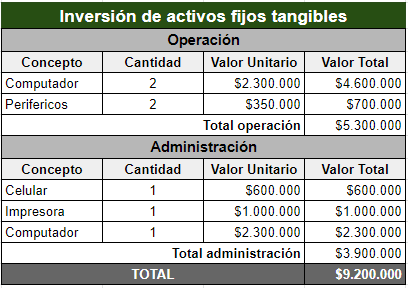
\includegraphics[width=0.7\textwidth]{Images/fijosTangibles.png}
\fnote{Nota. \textup{Fuente : Autores}}
\end{minipage}

\subsubsection{Activos fijos intangibles}

Los activos fijos intangibles se denominan a los procesos financieros y legales que la empresa debe tener en cuenta, descritos en la tabla \ref{activosIntangibles}.

\vspace{2mm}
\begin{minipage}{0.9\textwidth}
\centering
\captionof{table}[{ Inversión de activos fijos intangibles.}]{ Inversión de activos fijos intangibles. }
\label{activosIntangibles}
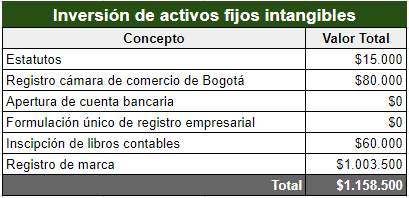
\includegraphics[width=0.7\textwidth]{Images/fijosIntangibles.png}
\fnote{Nota. \textup{Fuente : Autores}}
\end{minipage}

\subsubsection{Total activos fijos}
En la tabla \ref{totalActivos} se ilustra un resumen del total de inversión necesaria para adquirir los activos fijos y el capital de trabajado requerido para hacer el proyecto.

\vspace{2mm}
\begin{minipage}{0.9\textwidth}
\centering
\captionof{table}[{ Total activos fijos.}]{ Total activos fijos. }
\label{totalActivos}
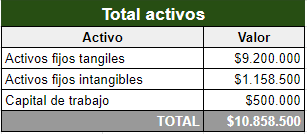
\includegraphics[width=0.7\textwidth]{Images/totalActivos.png}
\fnote{Nota. \textup{Fuente : Autores}}
\end{minipage}

\subsubsection{Financiamiento}
En la tabla \ref{financiacion} se ilustra la inversión que se debe hacer para la realización inicial del proyecto, esta debe analizarse tomando en cuenta el aporte social y el financiamiento de una entidad.

\vspace{2mm}
\begin{minipage}{0.9\textwidth}
\centering
\captionof{table}[{Financiación}]{ Financiación. }
\label{financiacion}
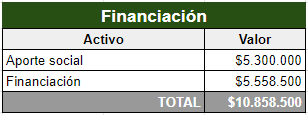
\includegraphics[width=0.7\textwidth]{Images/financiacion.png}
\fnote{Nota. \textup{Fuente : Autores}}
\end{minipage}